% Very simple template for lab reports. Most common packages are already included.
\documentclass[a4paper, 11pt]{article}
\usepackage[utf8]{inputenc} % Change according your file encoding
\usepackage{graphicx}
\usepackage{url}
\usepackage{listings}
\usepackage[justification=centering]{caption}

%opening
\title{Report 1: Rudy - a small web server}
\author{Emile Le Gallic}
\date{\today{}}

\begin{document}

\maketitle

\section{Introduction}

In this first homework we set up a small web server covering several topics :
\begin{enumerate}

    \item The HTTP protocol : how to parse HTTP request in order to extract the relevant fields of the request.
    \item The concept of a web socket : The \texttt{gen\_tcp} module provides an interface to TCP/IP sockets which allows us to open connections between two host and to exchange messages.  
\end{enumerate}

Furthermore, web servers are really related to distributed systems because they often need to handle many client requests concurrently, distribute workloads across multiple servers or nodes, and ensure high availability and fault tolerance. 


\section{Main problems and solutions}

In order to simulate a benchmark on several machines simultaneously, I wrote the \texttt{bench/4} function which is designed to measure the time it takes to execute a number of parallel requests to a server. It starts by recording the current time and then spawns multiple parallel processes (using \texttt{spawn\_parallel/4}) to handle the requests. After initiating these parallel processes, it waits for all of them to complete using \texttt{wait\_for\_parallel/1}. Finally, it calculates the elapsed time for the whole operation.

\hfill 

Initially, I encountered an issue with the run/4 function in the bench/4 implementation. The function used \texttt{self()} ! done to signal the completion of tasks. However, since \texttt{run/4} is executed within a spawned process, \texttt{self()} refers to that process rather than the parent process that initiated the parallel requests. This led to problems because the done message was not being sent to the correct process.

\hfill 

To resolve this, I modified the implementation to pass the \texttt{Parent} parameter (which is the parent process that originally called \texttt{bench/4}) to the \texttt{run/4} function. This way, the \texttt{run/4} function sends the done message to the correct parent process, ensuring that the \texttt{wait\_for\_parallel/1} function accurately waits for all child processes to complete. This adjustment ensured that the completion signals were received properly, allowing the \texttt{bench/4} function to correctly measure the total time for all requests.

\hfill

Also, as I was conducting experiments with several machines, and everything worked fine until I reached 7 machines; beyond that point, I encountered the error \texttt{\{error, etimedout\}} and \texttt{\{error, closed\}}. This error occurs because, with 7 machines running in parallel, the server struggles to handle the high number of simultaneous connections, leading to timeouts and closed connections. The server likely becomes overwhelmed due to resource constraints or network limitations, causing it to drop some requests or fail to respond in time, resulting in these errors.

\section{Evaluation}

\textit{If needed, you may provide figures or tables with main results
  evaluating your proposals. For each seminar, we will provide you
  with some guidance on which kind of evaluation you should do.}

I created a Python program that reads data from \texttt{experiment\_single.dat} and \texttt{experiment\_parallel.dat} files, calculates the average response time from the last three values of each line, and plots the server response time against delay time and the number of parallel processes, respectively, using \texttt{matplotlib}.

\hfill 

Here are the raw data and the plots :

\begin{table}[h]
\centering
\begin{tabular}{lcc}
Delay time (ms) & Average response time (µs) \\\hline
0 & 53796, 48950, 59911 \\\hline
10 & 1214230, 1214793, 1272529 \\\hline
20 & 2264821, 2279670, 2283438 \\\hline
30 & 3297435, 3237666, 3257649 \\\hline
40 & 4317210, 4299828, 4239350 \\\hline
50 & 5803364, 5283446, 5304433 \\\hline
100 & 10304341, 10264634, 10310753 \\\hline
200 & 20349431, 20320442, 20312783 \\\hline
300 & 30319490, 30334644, 30346009 \\\hline
\end{tabular}
\caption{
    Average response time for various server-side delay times (3 values computed for mean approximation)}
\label{tab:results}
\end{table}


\begin{center}
    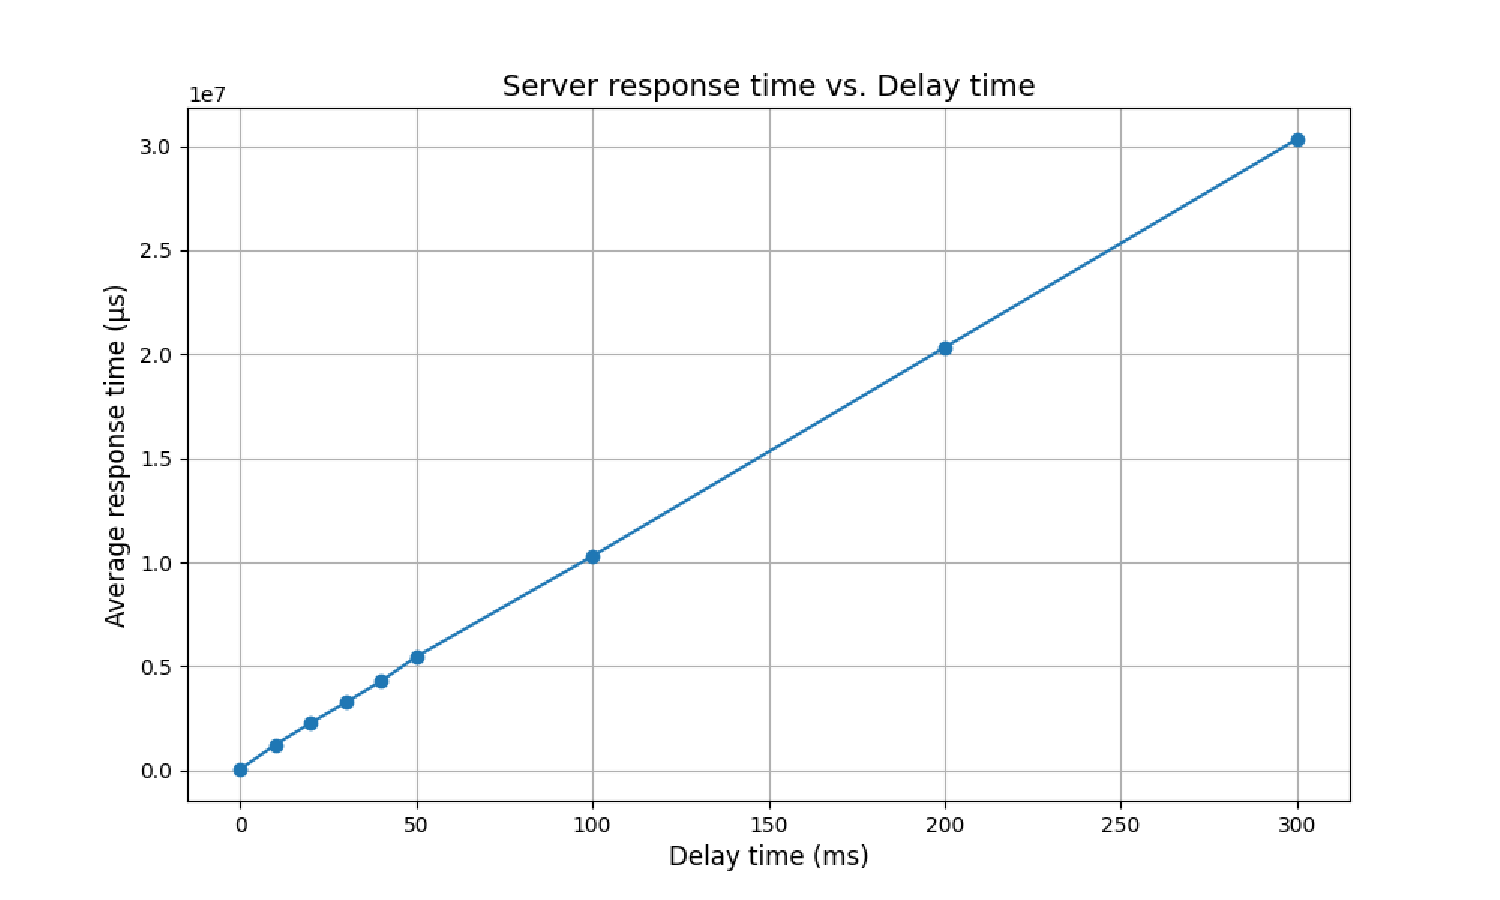
\includegraphics[scale=0.5]{result_single.pdf}
\end{center}

\begin{table}[h]
\centering
\begin{tabular}{lc}
Number of parallel processes & Average response time (µs) \\\hline
1 & 4231048, 4288257, 4249868 \\\hline
2 & 8224184, 8219808, 8246277 \\\hline
3 & 12346226, 12349116, 12345901 \\\hline
4 & 16468580, 16447298, 16459012 \\\hline
5 & 20579276, 20561990, 20554868 \\\hline
6 & 24669340, 24738464, 24701291 \\\hline
\end{tabular}
\caption{Average response time for varying numbers of parallel processes (3 values computed for mean approximation)}
\label{tab:parallel_results}
\end{table}


\begin{center}
    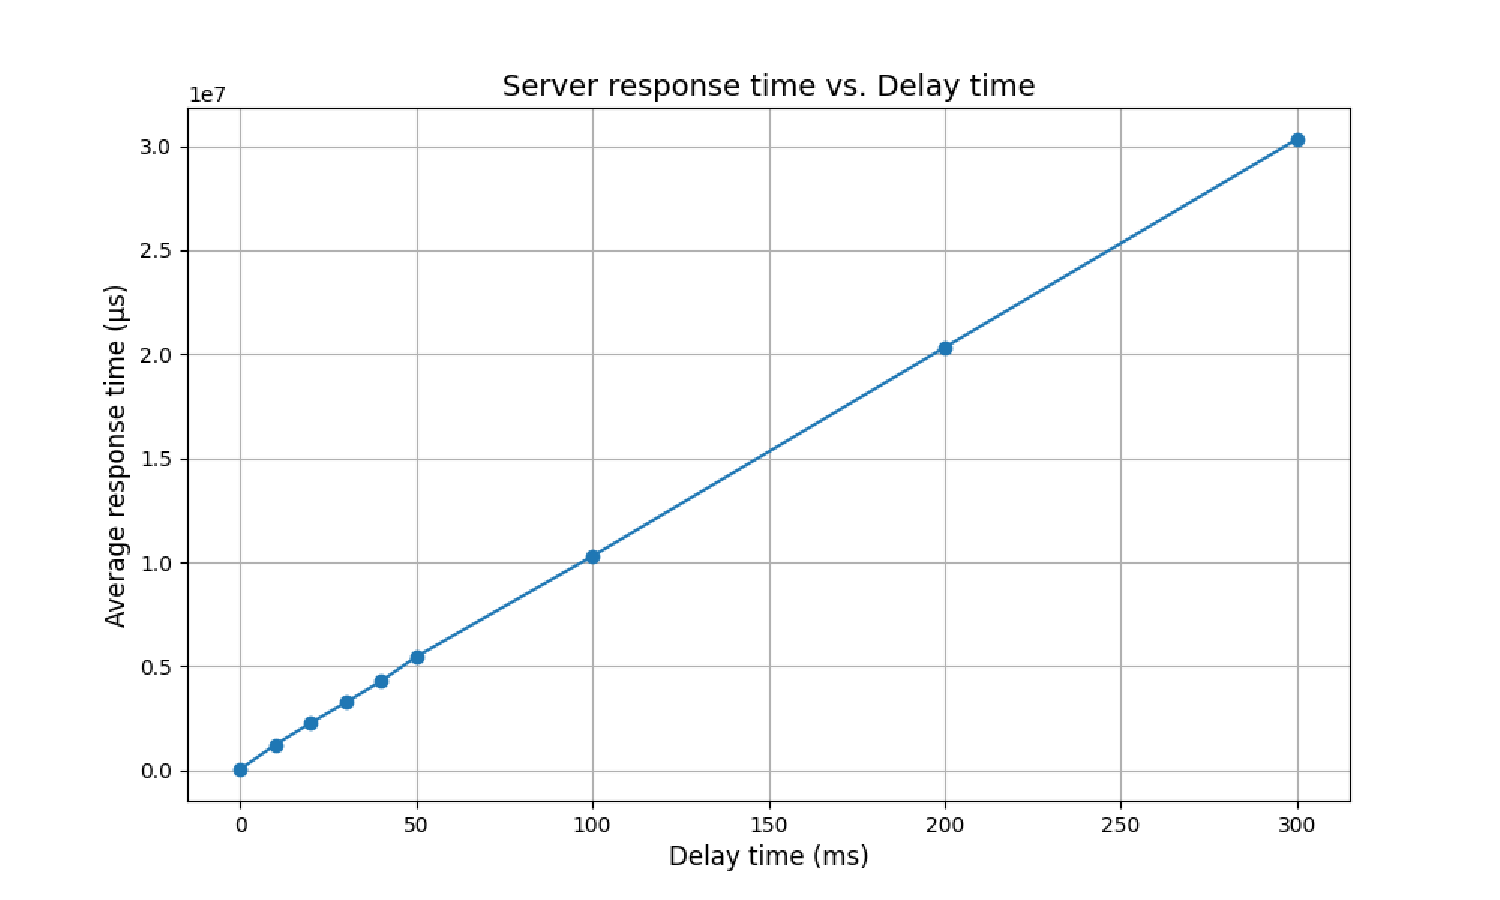
\includegraphics[scale=0.5]{result_single.pdf}
\end{center}


\section{Conclusions}

\textit{Change the layout of this template as you want. It's only for
  your guidance but if you feel that you need a different structure,
  feel free to change it. The report should not be too long ($\approx
}

What have you learnt from the problem presented?
Was it useful?


\end{document}
